% !Mode:: "TeX:UTF-8"
\chapter{开发环境}
\label{chap:java_dev_environment}

本书主要介绍\gls{AI}在Java语言上的应用,第一部分内容专为没有编程基础的同学准备,如果你已经具备一定的编程能力可从第二部分开始阅读。
下面先介绍本书所需要的开发环境,如果你已配置,也可跳过本章内容。

自从1996年诞生第一个Java版本以来,已经发布过很多版本,每个版本都会多少引入一些新的语法和功能。
本书所提供的示例,都可以在JDK7+上顺利运行,用到开发工具有\tabref{tab:part1_dev_env}:

\begin{table}[!htbp]\centering
\small
\begin{tabular}{|p{4cm}|p{8cm}|}
\hline
\multicolumn{2}{|c|}{开发环境}\\
\hline
1.JDK8+&最新版本是JDK10,可以尝试\\
\hline
2.IntelliJ IDEA&友好的界面,强大的编程环境\\
\hline
3.Eclipse&不建议使用\\
\hline
4.jupter&适合验证代码,打开网页就可编码\\
\hline
5.ND4J&强大的运算Java库\\
\hline
6.DL4J&深度学习Java库\\
\hline
\end{tabular}
\caption{开发环境}
\label{tab:part1_dev_env}
\end{table}

\section{安装JDK}
安装JDK(Java Development Kit)的时候,我们有2个选择:Oracle JDK和OpenJDK。
经过很多用户验证和测试,你基本可以无视两者之间的差异。
使用Linux系统的同学,建议保持默认的OpenJDK。

Sun在1998成立JCP(Java Community Process)控制Java的开发节奏,任何想要加入的Java功能和特性,都必须以JSR(Java Specification Request)正式文件的方式提交。
然后JSR经过JCP执行委员会投票通过之后,才可成为最终的标准,有能力的厂商或组织可以根据JSR实现JDK。
从2006年Sun开源JDK之后,很顺利地出现了OpenJDK,它是一个对商业友好的版本。
Oracle在收购Sun之后,重申对JDK的服务费用。实际上,Sun在被收购之前就开始索要授权费,但始终没有强制收取。
而Oracle与Google Android之间的JDK纠纷加重了产商对JDK的忧虑。
Oracle Java并不是完全免费的,要注意其中的收费条款。

\begin{itemize}
\item[1.]http://openjdk.java.net/install/
\item[2.]http://www.oracle.com/technetwork/java/javase/downloads/index.html
\end{itemize}

\noindent
注意JDK和JRE的区别,JRE(Java Runtime Environment)是Java程序的运行环境,不要下载错了。
安装JDK的过程中,全部默认点选“下一步”即可。
若在安装过程中,没有添加到环境变量的选项,就需要我们手动配置以下2个环境变量。

\begin{itemize}
\item[1.]JAVA\_HOME
\item[2.]CLASSPATH
\end{itemize}

\emph{环境变量}实际上是一种系统变量,方便计算机的软件之间共享配置的方法。
有些计算机上安装的Java可能不止一个,配置不同的JAVA\_HOME就能切换JDK版本。
如\figref{fig:part1_java_home}。

\begin{figure}[!htb]
\centerline{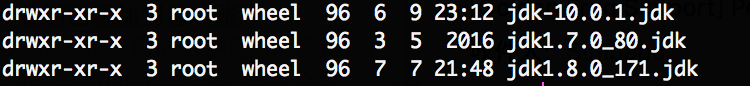
\includegraphics{images/java_home.png}}
\label{fig:part1_java_home}
\caption{Java路径}
\end{figure}

配置JAVA\_HOME非常简单,把它指向对应JDK的安装路径就可,不同操作系统有些差异,在此不再赘述。

而CLASSPATH这个环境变量,如果使用IDE开发环境也可以不配置。
如果你的Java程序依赖第三方Jar,不配置CLASSPATH就有可能找不到对应的class。
关于\emph{class not found}这种问题,\chapref{chap:java_datatype}会对此进行说明。这里先告诉大家有这个事情,暂时先不配置。

\section{集成开发环境}
现代化软件开发,离不开IDE(集成开发环境)的支持。
好用的IDE不仅有助于提高编码效率,还可以辅助检查错误,集成项目管理等功能。
主流的Java开发环境有Eclipse、IDEA(社区版本免费)和VS Code,根据个人喜好选择一个即可。
本书例子全部在IDEA上验证通过。

\begin{figure}[!htb]
	\centering
	\begin{minipage}{0.2\textwidth}
		
\includegraphics[width=2cm]{images/logo_eclipse.png} \\
		\centering Eclipse
	\end{minipage}
	\begin{minipage}{0.2\textwidth}
		
\includegraphics[width=2cm]{images/logo_vscode.png} \\
		\centering VS Code
	\end{minipage}
	\begin{minipage}{0.2\textwidth}
		
\includegraphics[width=2cm]{images/logo_idea.png} \\
		\centering IDEA
	\end{minipage}
\end{figure}

\noindent
使用IDEA,在官网(https://www.jetbrains.com/idea/)下载社区版本安装即可。
软件开发过程,也离不开版本控制(Revision control)工具,用于记录一个或多干文件的变化,
方便以后查阅特定版本修订情况。
最重要的一点,可以使多人协作完成软件开发,确保不同人所编辑的同一档案都是最新的。
Git是目前最流行的版本控制工具,可以在https://git-scm.com/downloads下载安装。
然后,打开IDEA配置界面检查Git的路径是否正确,修改之后就可以使用了。
(Settings->Version Control->Git)

\section{配置DL4J环境}
DeepLearning4J(DL4J)是一套基于Java语言的神经网络工具包,可以构建、定型和部署神经网络。
DL4J与Hadoop和Spark集成,支持分布式CPU和GPU,为商业环境(而非研究工具目的)所设计。
Skymind是DL4J的商业支持机构。
DL4J包括了分布式、多线程的深度学习框架,以及普通的单线程深度学习框架。
定型过程以集群进行,也就是说,Deeplearning4j可以快速处理大量数据。

本书从理论出发,结合DL4J的示例由浅入深地介绍机器学习知识。
示例项目由Maven进行构建和依赖管理,基于项目POM(对象模型)定义项目的基本信息,
用于描述项目如何构建,声明项目依赖等。
\footnote{Maven 曾是 Jakarta 项目的子项目,现为由 Apache 软件基金会主持的独立 Apache 项目。}
具体的IDEA项目配置方法,可参考DL4J官网给的建议:

\begin{enumerate}
	\item Java (SDK) 1.7之后的版本 (限64位)
	\item Apache Maven (自动编译和依赖管理)
  \item IntelliJ IDEA 或 Eclipse
  \item Git
\end{enumerate}

\begin{lstlisting}
$ git clone https://github.com/deeplearning4j/dl4j-examples.git
$ cd dl4j-examples/
$ mvn clean install
\end{lstlisting}